%
% Chapter 4
%

\chapter{DISCUSSION AND INTERPRETATION}\label{chp:discussion}

% When reporting the lifetimes in this work, it is prudent to distinguish which angular distribution is used, as the lifetimes are sensitive to inflation from multiple sources. First, recall Figure \ref{fig:ftau_all}, where we observe inflation of the lifetimes due to the calculation of \textit{F}($\tau$) from a higher neutron energy, and thus, a modified value for the nuclear and electronic stopping powers that allows us to extract the lifetime. Second, the extracted lifetime can be inflated due to level-feeding effects from higher-lying excitations in the nucleus; for these reasons, we want to report lifetimes from the \textit{lowest} energy threshold possible to reduce the effect of this lifetime inflation. An example of the proportional lifetime inflation for two excited states caused by level-feeding and bombarding neutron energy differences can be seen in Figure \ref{fig:lifetime_inflation}. 
% 
% \begin{figure}[h!]
% \begin{center}
% 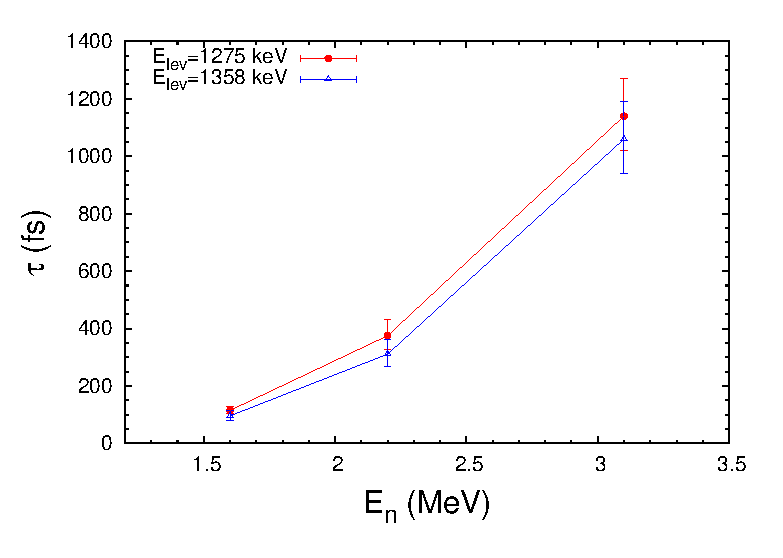
\includegraphics[width=0.85\textwidth]{lifetime_inflation_example.eps}
% \caption{Lifetime inflation of the measured lifetimes for two levels (E$_{lev}$=1275~keV and E$_{lev}$=1358~keV) in $^{162}$Dy caused by effects due to a higher bombarding neutron energy and level-feeding. \label{fig:lifetime_inflation}}
% \end{center}
% \end{figure}

%Discussion introduction HERE

Lifetimes of the 13 positive parity states belonging to 4 positive parity bands and 11 negative parity states across the 4 negative parity bands in $^{160}$Gd are discussed in this chapter, along with the 19 positive parity states spread across 9 positive parity bands and 18 negative parity states belonging to 7 negative parity bands in $^{162}$Dy. Lifetimes are converted to transition probabilities in Weisskopf units to provide context to the transition rates between any collective states observed. Unless otherwise noted, transition probabilites are deduced from the experimentally measured quantities ($\gamma$-ray energies, $\gamma$-ray intensities, lifetimes, multipole mixing fractions, and associated measured uncertainties); particular cases where we do not observe a $\gamma$ ray, and thus do not have intensities, energies or mixing information, use literature decay information where available (these cases are explicitly stated).


\section{$^{160}$Gd Discussion}



\subsection{Excited 0$^+$ States and the K$^\pi$=2$^+_\gamma$ Band}

The 0$^+$ excitations in $^{160}$Gd serve to highlight some of the distinct advantages of (n,n$^\prime\gamma$) studies performed at UKAL. Previous literature assertions list four 0$^+$ excitations in $^{160}$Gd, from various experiments, two of which are tentative assignments \cite{Berzin_160Gd_reject0,Lovhoiden_160pt}. In \cite{Lesher_160Gd0s}, we exploit two facets from the angular distribution and excitation function measurements to rule out the two tentative assignments. First, angular distributions for $\gamma$ radiation leaving a 0$^+$ state must be isotropic, and secondly, that energy thresholds of a $\gamma$-ray leaving a 0$^+$ state will come in at precisely the level energy (recall that there is no extra energy needed to make non-zero angular momentum transfers). 

The previous assignment of a 0$^+$ excitation at E$_{lev}$=1325.73~keV was made by \cite{Berzin_160Gd_reject0} in a (n,n$^\prime\gamma$) reaction using continuous energy reactor neutrons, with a refutation of this assignment made in this work and by angular distribution measurements performed in \cite{Govor_160Gd_2009}. The justification for this refutation of a J=0 assignment is shown in Figure \ref{fig:160Gd_1250_noniso}, a clearly anisotropoic angular distribution of the E$_\gamma$=1250.4~keV de-excitation, explicitly stating that this radiation cannot stem from a 0$^+$ excitation. A similar check was made via the normalization of angular distributions; absolute intensities of $\gamma$ rays were normalized so that radiation from the lowest-lying 0$^+$ state is isotropic. In the case where we used a normalization to this E$_\gamma$=1250.4~keV $\gamma$ ray, angular distributions of well-behaved dipole and quadrupole radiation (\textit{e.g.} E2 radiation from strong ground-state band transitions) ceased to exhibit the expected behavior of a classically oscillating charge distribution from Figure \ref{fig:multipole_diff}. Contrast this catastrophic result from this normalization attempt to the one in use by normalizing to the E$_\gamma$=1304.46~keV from the 1379~keV state, and we see the return of `concave-up' angular distributions for quadrupole radiation, leaving us with a clear choice for normalization and furthermore pointing away from the assignment of the 1325~keV state as a 0$^+$ excitation.

\begin{center}
\begin{figure}[h!]
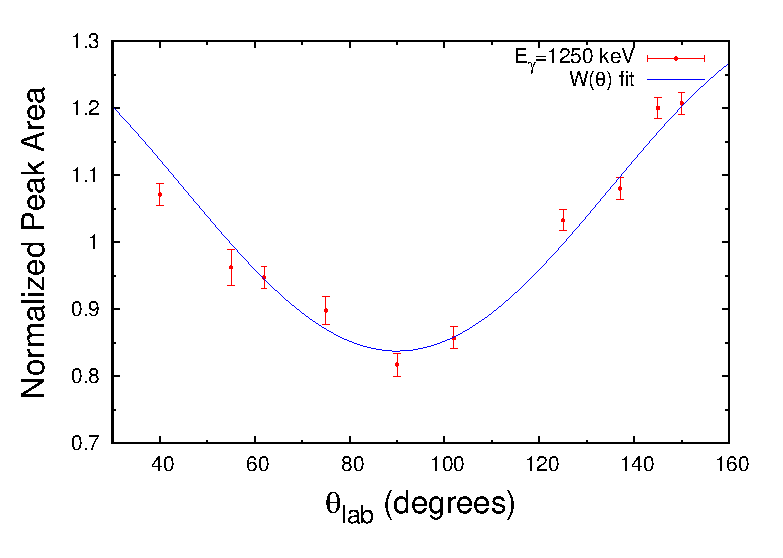
\includegraphics[width=0.99\textwidth]{figures/1250_Gd.eps}
\caption{Non-isotropic decay from the tentative 0$^+$ state in $^{160}$Gd at E$_{\rm x}$=1325~keV. \label{fig:160Gd_1250_noniso}}
\end{figure}
\end{center}

The second tentative 0$^+$ excitation at E$_{lev}$=2236~keV was placed in \cite{Lovhoiden_160pt} via a (t,p) transfer reaction study; we also reject this assignment based on, again, the non-isotropic nature of $\gamma$-radiation from the single observed E$_\gamma$=2162.74~keV de-excitation, as well as a threshold energy below that of the excitation energy of the state. This creates a completely illogical and unphysical system, where a $\gamma$-ray is populated below the energy of the state, and as such, cannot be attributed to this excitation. The excitation function measurement for this decay can be seen in Figure \ref{fig:160Gd_2163_exfGd}, with a threshold clearly below 2100~keV.

\begin{center}
\begin{figure}[h!]
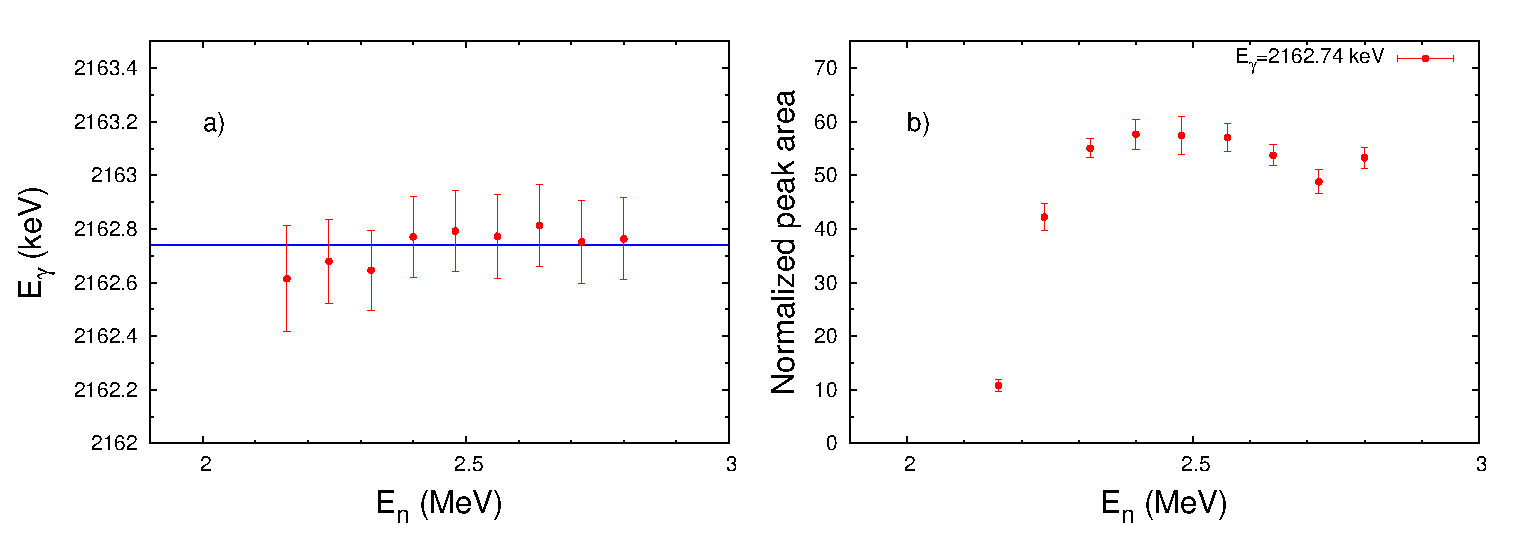
\includegraphics[width=0.99\textwidth]{figures/2163_exfGd.eps}
\caption{Excitation function measurement from the tentative 0$^+$ state in $^{160}$Gd at E$_{\rm x}$=2236~keV. \label{fig:160Gd_2163_exfGd}}
\end{figure}
\end{center}

This leaves only two 0$^+$ excitations remaining in $^{160}$Gd as candidates for either a single-phonon $\beta$ vibration or a double-phonon ($\gamma\gamma$, double octupole, etc) type, now labeled as the 0$^+_2$ and 0$^+_3$ bands.  A corresponding level scheme with the decays out of K$^\pi$=0$^+$ bandmembers is shown in Figure \ref{fig:160Gd_0s}. 

\begin{center}
\begin{figure}[h!]
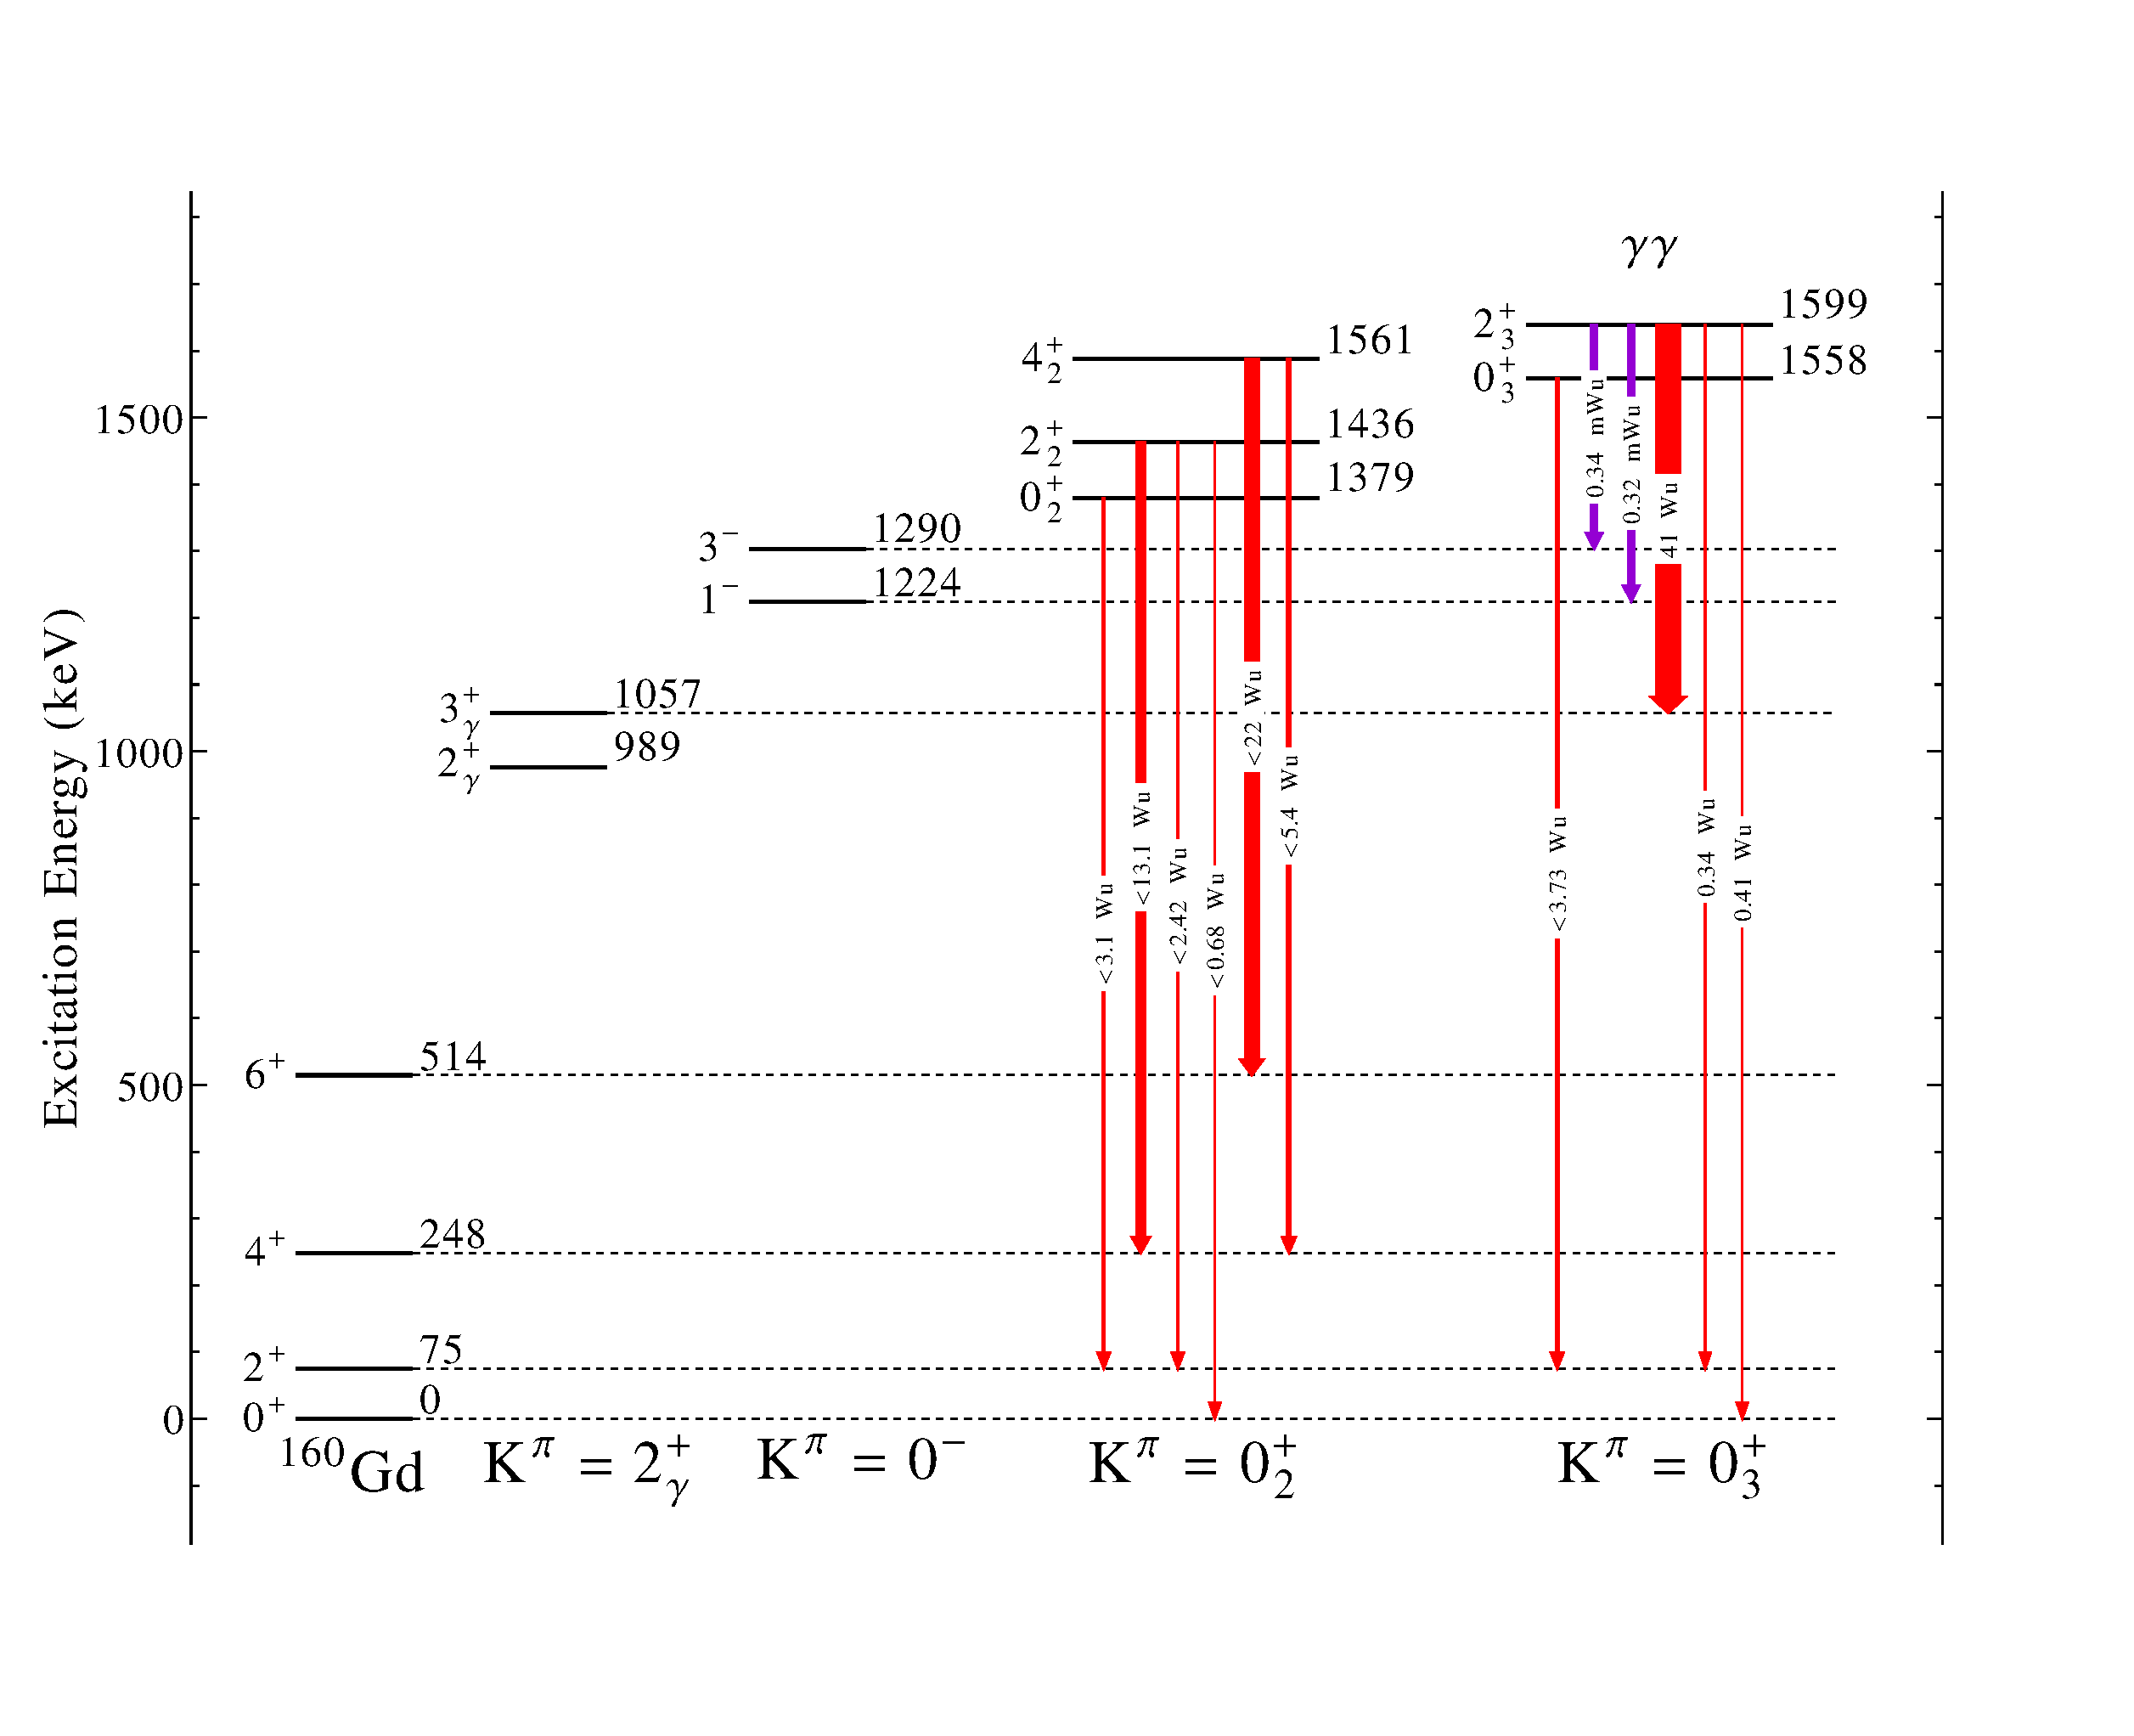
\includegraphics[width=0.99\textwidth]{figures/160Gd_Partial0sRevised.pdf}
\caption{Level scheme showing the calculated B(E2) in W.u. and B(E1) in mW.u. for the confirmed 0$^+$ excitations in $^{160}$Gd.
\label{fig:160Gd_0s}}
\end{figure}
\end{center}

Six (6) $\gamma$ rays were detected to determine the lifetimes of three levels in the K$^\pi$=0$^+_2$ band in our $^{160}$Gd(n,n$^\prime\gamma$) experiments. Decays leaving the 0$^+_2$ band display varying levels of collectivity based off our lower-limit lifetime measurements in the band (at least $>$320~fs for each state). In terms of offering a concrete case for assessing this band as a $\beta$-vibration, we can tentatively point to this band as a single-phonon quadrupole vibration from its potentially strong transition probabilities to the ground state (or from our measurement of upper limits on the collectivity). Given the limitations of what lifetimes DSAM can measure, we are left with an obviously murky picture for any possible $\beta$-vibration in $^{160}$Gd due to our measurement of lifetime limits, although the potentially collective decays to the ground state tend to suggest some (albeit weak) $\beta$-vibrational interpretation of this band at E$_{\rm x}$=1379~keV. Due to the lack of intraband transitions observed in our experiment, we cannot place any two-phonon characteristics to this set of excitations, as we should expect strong B(E2) values connecting the 0$^+_2$ band to the 2$^+_\gamma$ band at E$_{\rm x}$=988~keV. An ideal situtation for further study includes the refinement of the lifetime measurements of this band via another measurement technique to concretely assign a $\beta$-vibration to this band, as the collective upper limit is \textit{indicative} of a $\beta$-vibration, but is not conclusive enough to say for certain. 
%[OFFER SOME INTERPRETATION, DISAPPEARING 0+ STRENGTH, VIABILITY OF THE 0_2 AS A BETA VIBRATION,ETC, this likely goes better in the implications section]

A similar, yet also contrasted story emerges with the discussion of any single-phonon characteristics in the 0$^+_3$ band at E$_{\rm x}$=1558~keV; six (6) $\gamma$ rays were detected to measured the lifetime of two states in the K$^\pi$=0$^+_3$ band. The decays to the ground state exhibit characteristically weak collectivity ($<$4~W.u. for the bandhead and $<$0.5~W.u. for the 2$^+$ member), pointing away from the interpretation as a $\beta$-vibration. However, the refinement of the 1599~keV state's lifetime opens up key discussion for the 0$^+_3$ band. We have measured a $\gamma$ ray that corresponds to an intraband transition, namely to the K$^\pi$=2$^+$ $\gamma$-vibrational band, with an inflated B(E2) value of 41$^{+16}_{-37}$~Weisskopf units. While the uncertainty of this transition probability is large due to the measured lifetime's uncertainty, this strong, preferential decay is indicative of signatures for the antialigned (K=0) double-phonon $\gamma\gamma$-vibration. Our measurement of the angular distribution for this $\gamma$ ray led to our overhwelmingly E2-type mixing ratio ($\delta$=-5.57$^{+1.91}_{-5.00}\rightarrow$96.8\% E2). Of further note, the 0$^+_3$ band displays some slightly inflated transition probabilities to the lowest lying K$^\pi$=0$^-$ band at $\sim$0.3~mW.u. strength. These somewhat inflated B(E1) probabilities would otherwise be indicative of some double-octupole phenomena in the nucleus, but with the presence of the extraordinarily large B(E2) to the $\gamma$-vibrational band, more interest and a higher feasability is placed on the interpretation of this band as a double quadrupole vibration (K$^\pi$=0$^+$, $\gamma\gamma$-type). 
% \subsection{K$^\pi$=2$^+_\gamma$ band}

Staying within the same vein of quadrupole excitations, we turn our attention to any $\gamma$-vibrational characteristics of $^{160}$Gd. While the nature of K$^\pi$=2$^+$ bands is not as heavily debated as the 0$^+$ bands \cite{McGowan_BE2_1981,Burke_hexadecapole1994,PhysRevC.54.679,JAMMARI_1988}, our lifetime measurements of the states in this $\gamma$-vibrational band warrant discussion, as any collective excitations built on-top of this band should be a multiphonon configuration. The decays observed from the lowest K$^\pi$=2$^+_\gamma$ band are shown in Table \ref{tab:160Gd_gamma} and Figure \ref{fig:160Gd_Octupole}. Overall, we see systematically expected behavior (inflated levels of collectivity averaging about 5-10~W.u.) in terms of the strength of the other 2$^+_\gamma$ excitations in the rare-earth region of nuclei \cite{McGowan_BE2_1981,GROTDAL1968385,MCGOWAN_168Er_E3,KORTEN_1993}, and as such, we can assign and confirm this band as a quadrupole $\gamma$-vibration in $^{160}$Gd. Generally, it is prudent to obtain this base-level of collectivity in the nucleus to compare the feasability of other phonon excitations, or to make claims on any two-phonon characteristics in $^{160}$Gd. We are yet again presented with the well-behaved $\gamma$-vibration that has stood the test of time for and has been a figurehead in nuclear structure in deformed rare-earth nuclei.

\subsection{Negative Parity States}\label{sec:160Gd_negparity}
The determination of any reflection-asymmetry and thus, potential octupole shape correlations in $^{160}$Gd will lie in the measurement of B(E1) transition probabilities of de-excitations from the low-lying negative parity states. The decays from all observed negative parity bands in $^{160}$Gd are shown in Figure \ref{fig:160Gd_Octupole} alongside the K$^\pi$=2$^+_\gamma$ decays from the previous section. The tabulated results from all E1 decays observed in the experiments can be seen in Table \ref{tab:160Gd_negparity}.

\begin{center}
\begin{figure}[h!]
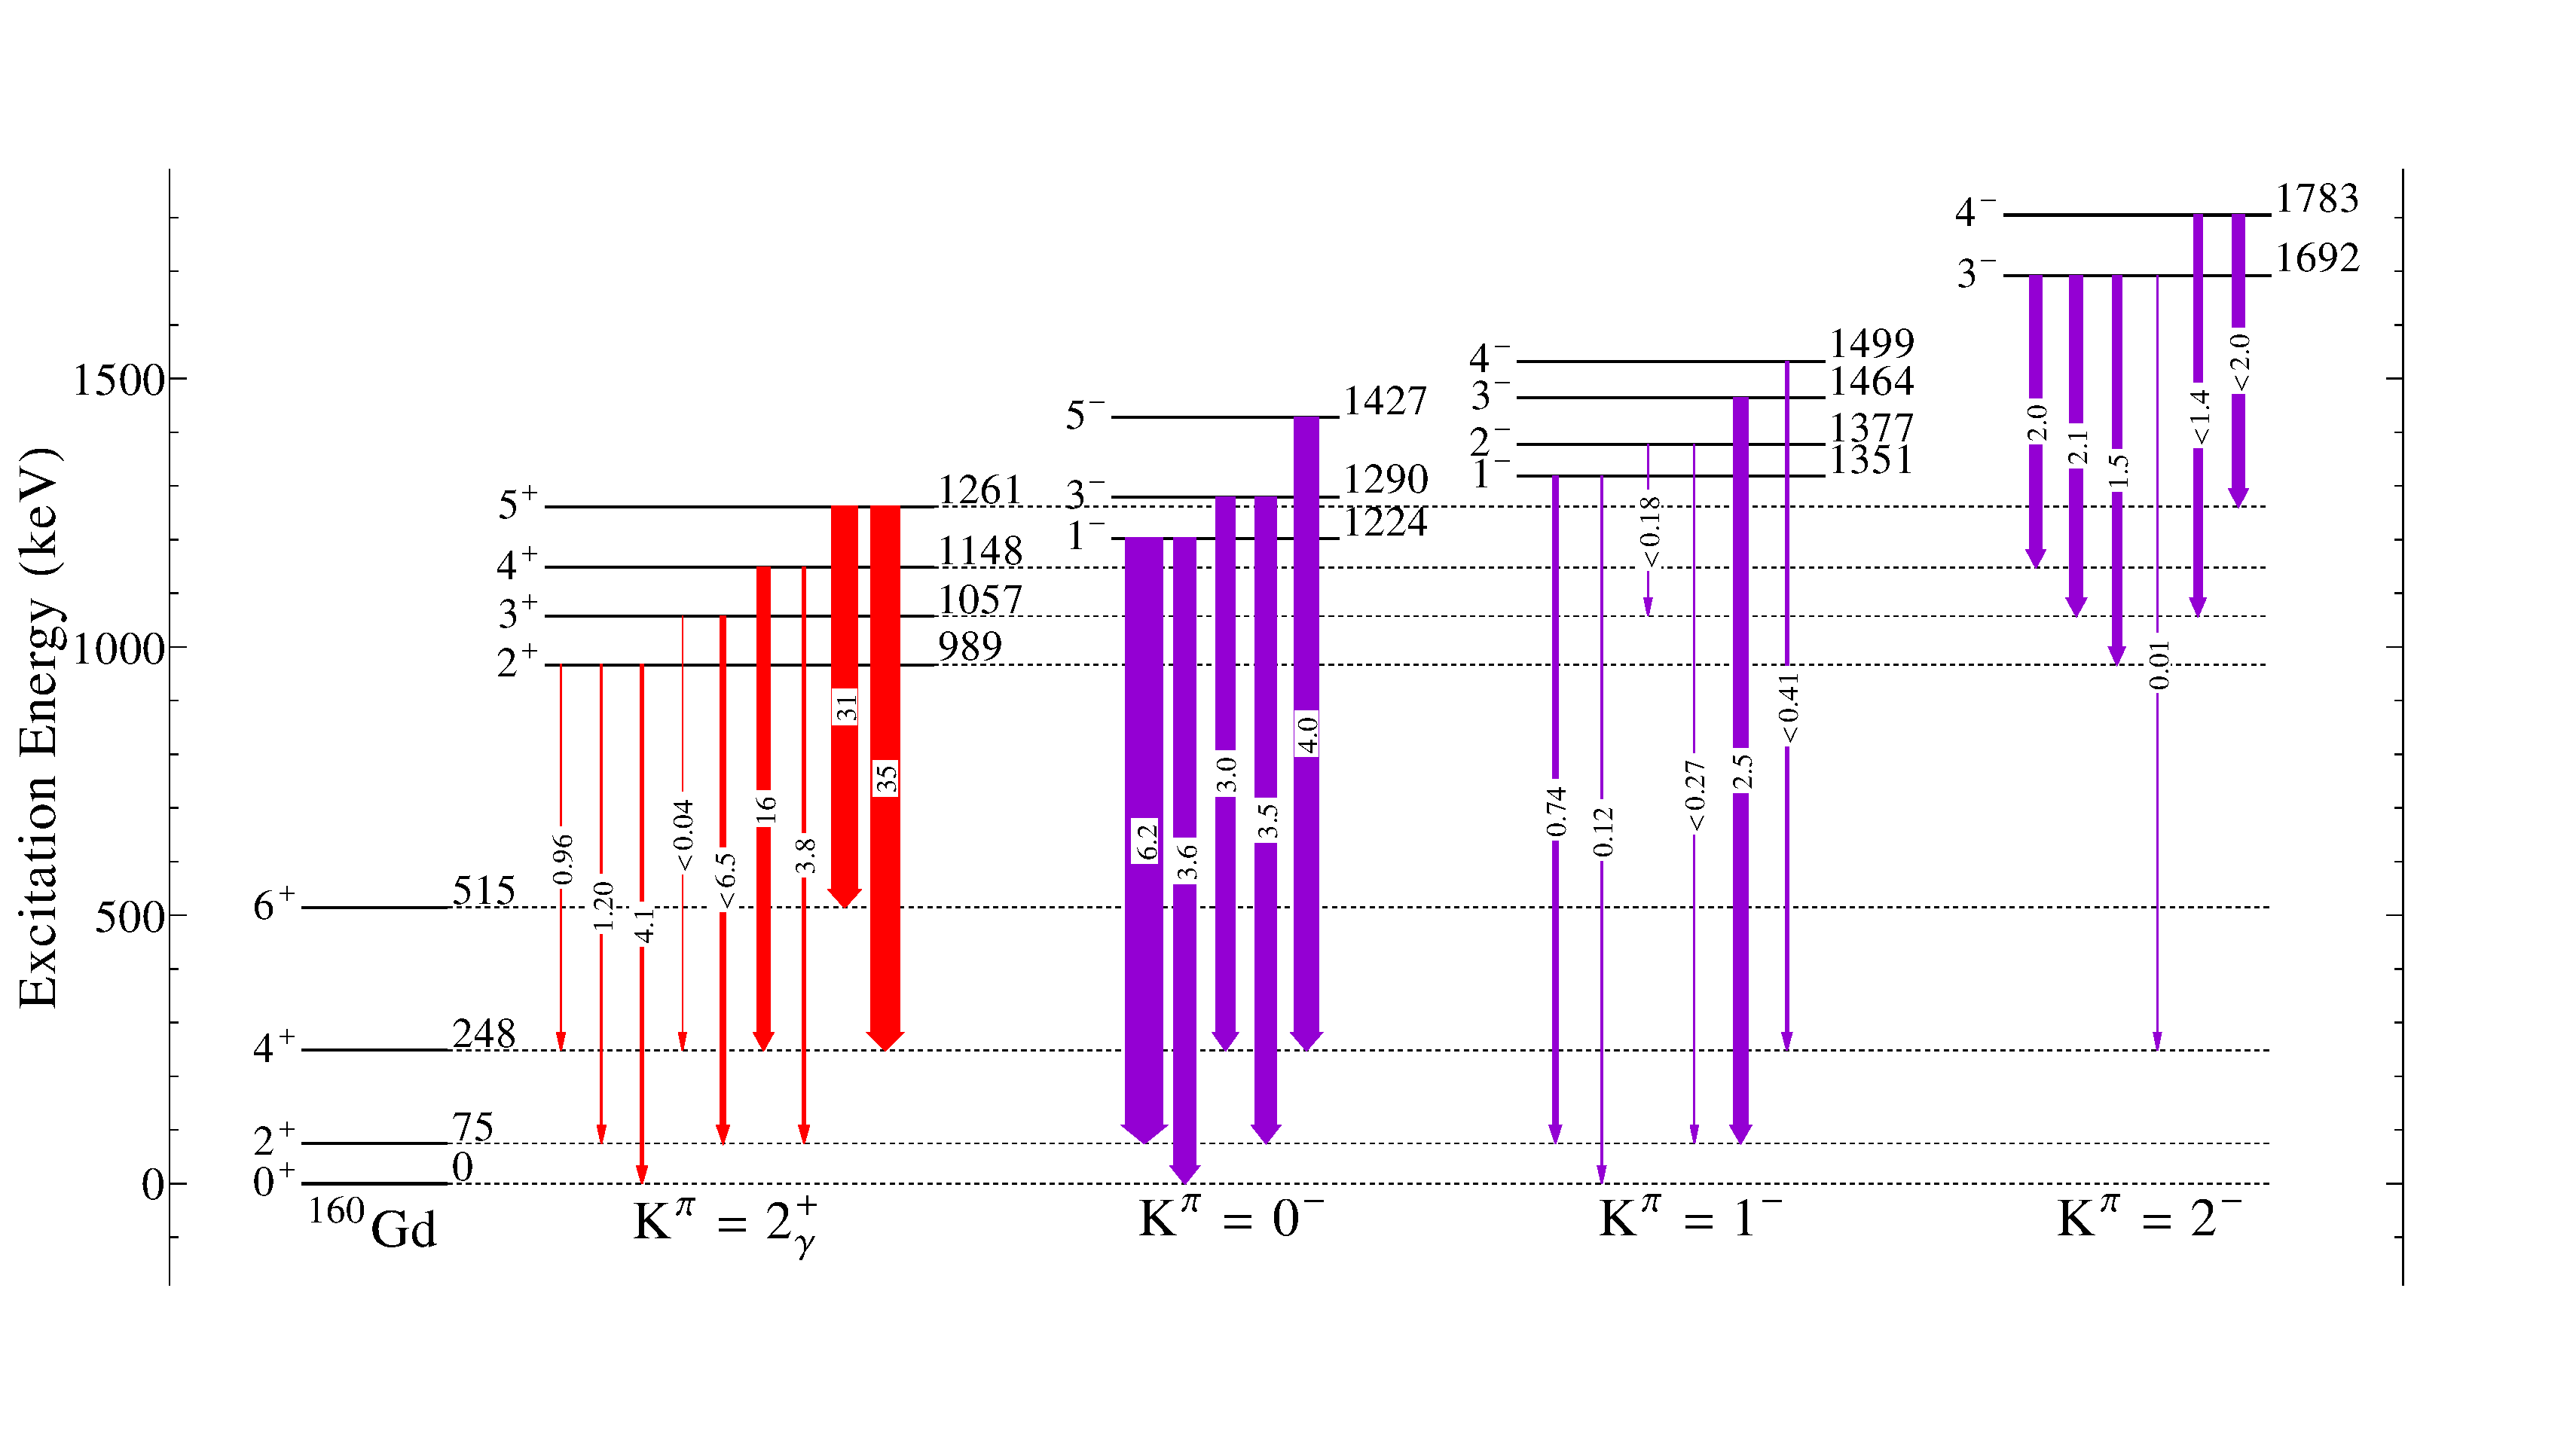
\includegraphics[width=0.99\textwidth]{figures/160Gd_OctupoleRevised.pdf}
\caption{Level scheme showing the decays with calculated reduced transition probabilities for the K$^\pi$=2$^+_\gamma$ band and low-lying negative parity states in $^{160}$Gd. \label{fig:160Gd_Octupole}}
\end{figure}
\end{center}                                    
                                                

 The deduced B(E1)s from the K$^\pi$=0$^-$ band show large inflation of collectivity from these states, strongly indicating a well-behaved octupole vibration in $^{160}$Gd. This octupole collectivity in the B(E1)s are corroborated by the experimentally measured and distinctly collective B(E3;0$^+\rightarrow$3$^-$) transition probability (0.118(7)~e$^2$b$^3$) by \cite{McGowan_BE2_1981}.
%0- band acts like a wellbehaved octupole vibration, enhanced E1s, discuss these 
%B(E3;0->3)=0.120 (6)

%1- band likewise, looks like it belongs to the standard octupole vibration mentioned in theory, GOVOR nnp work assigned these spins and parities.
 We also measure comparably short lifetimes for two of the four members that result in distinctly collective (yet not as collective as the K$^\pi$=0$^-$ band), indicating that this band could indeed be a part of the fragmented octupole vibration in $^{160}$Gd. The shallow values for F($\tau$) in this state cannot offer a concrete idea of the collectivity of the state. A similar argument applies for the 4$^-$ state at 1498~keV, where we only observe a shallow shift from the Doppler plots; luckily, these other members of the 1$^-$ band can offer some insight from the well-defined lifetime measurements. Overall, the observation of moderately inflated levels of collectivity in the band seems to indicate that these rotational members of the K$^\pi$=1$^-$ band are indeed a part of the octupole vibration.

%begs the question, where is the 3- band? OR where is the 2- band if the states at 1691 aren't actually a 2- band


% L$\o$vh$\o$iden \cite{Lovhoiden_160pt} 

 We measure distinct collectivity from the 3$^-$ member of the K$^\pi$=2$^-$ band connecting to the $\gamma$-vibrational band, following a recent trend of observation by \cite{Pascu_octupole_2015,Spiecker_E1strength} of strong E1 radiation in 2$^-\rightarrow$2$^+$ transitions. The same trend of (potentially) collective E1s to the $\gamma$-vibrational band occur in the 4$^-$ member of the band, where we only have a lower limit to the lifetime. This is obviously a curious behavior and needs more work to assign any conclusive detail to the rotational band. B(E3) transition probabilities to the $\gamma$-band are critical in achieving this goal; barring those measurements, only the ideas presented in current, developing works can be applied, but this is still a significant contribution to the total E1 strength in deformed nuclei, whether or not it is a part of the octupole vibration. Furthermore, we can safely adopt this K$^\pi$=2$^-$ assignment from the well-behavedness and agreement of the deduced B(E1)s in comparison to the Alaga rules (Table \ref{tab:160Gd_ALAGA}).
% OFFER INTERPRETATION HERE MODIFIED FROM THE SECOND 160GD PAPER


Our measurement of lifetimes in the lowest-lying negative parity bands begs the question: where is the 3$^-$ member of the traditional octupole multiplet? Or at least, if this band is \textit{not} the K$^\pi$=2$^-$ band and instead the K$^\pi$=3$^-$ band, where is the missing part of the octupole quartet of states? Population of $\Delta$K=3 states is difficult (but not impossible) to accomplish with (n,n$^\prime\gamma$) reactions, but the states would be very weak, and we may simply lack the statistics needed to observe such states with any reliability. In a soon to be echoed tone throughout this work, more senstitive experiments (or much higher statistics in terms of beam time, reaction rates, etc) are needed to have fully spectroscopy and measurement of lifetimes in $^{160}$Gd. Especially from our observation of negative parity states that do not decay strongly to the ground state (the K$^\pi$=2$^-$ band), the traditional picture of fragmented octupole collectivity seems tentative as we approach the rotational limit (R$_{\frac{4}{2}}\sim$3.3).
\subsection{Other Lifetime Measurements in $^{160}$Gd}


\begin{center}
\begin{figure}[h!]
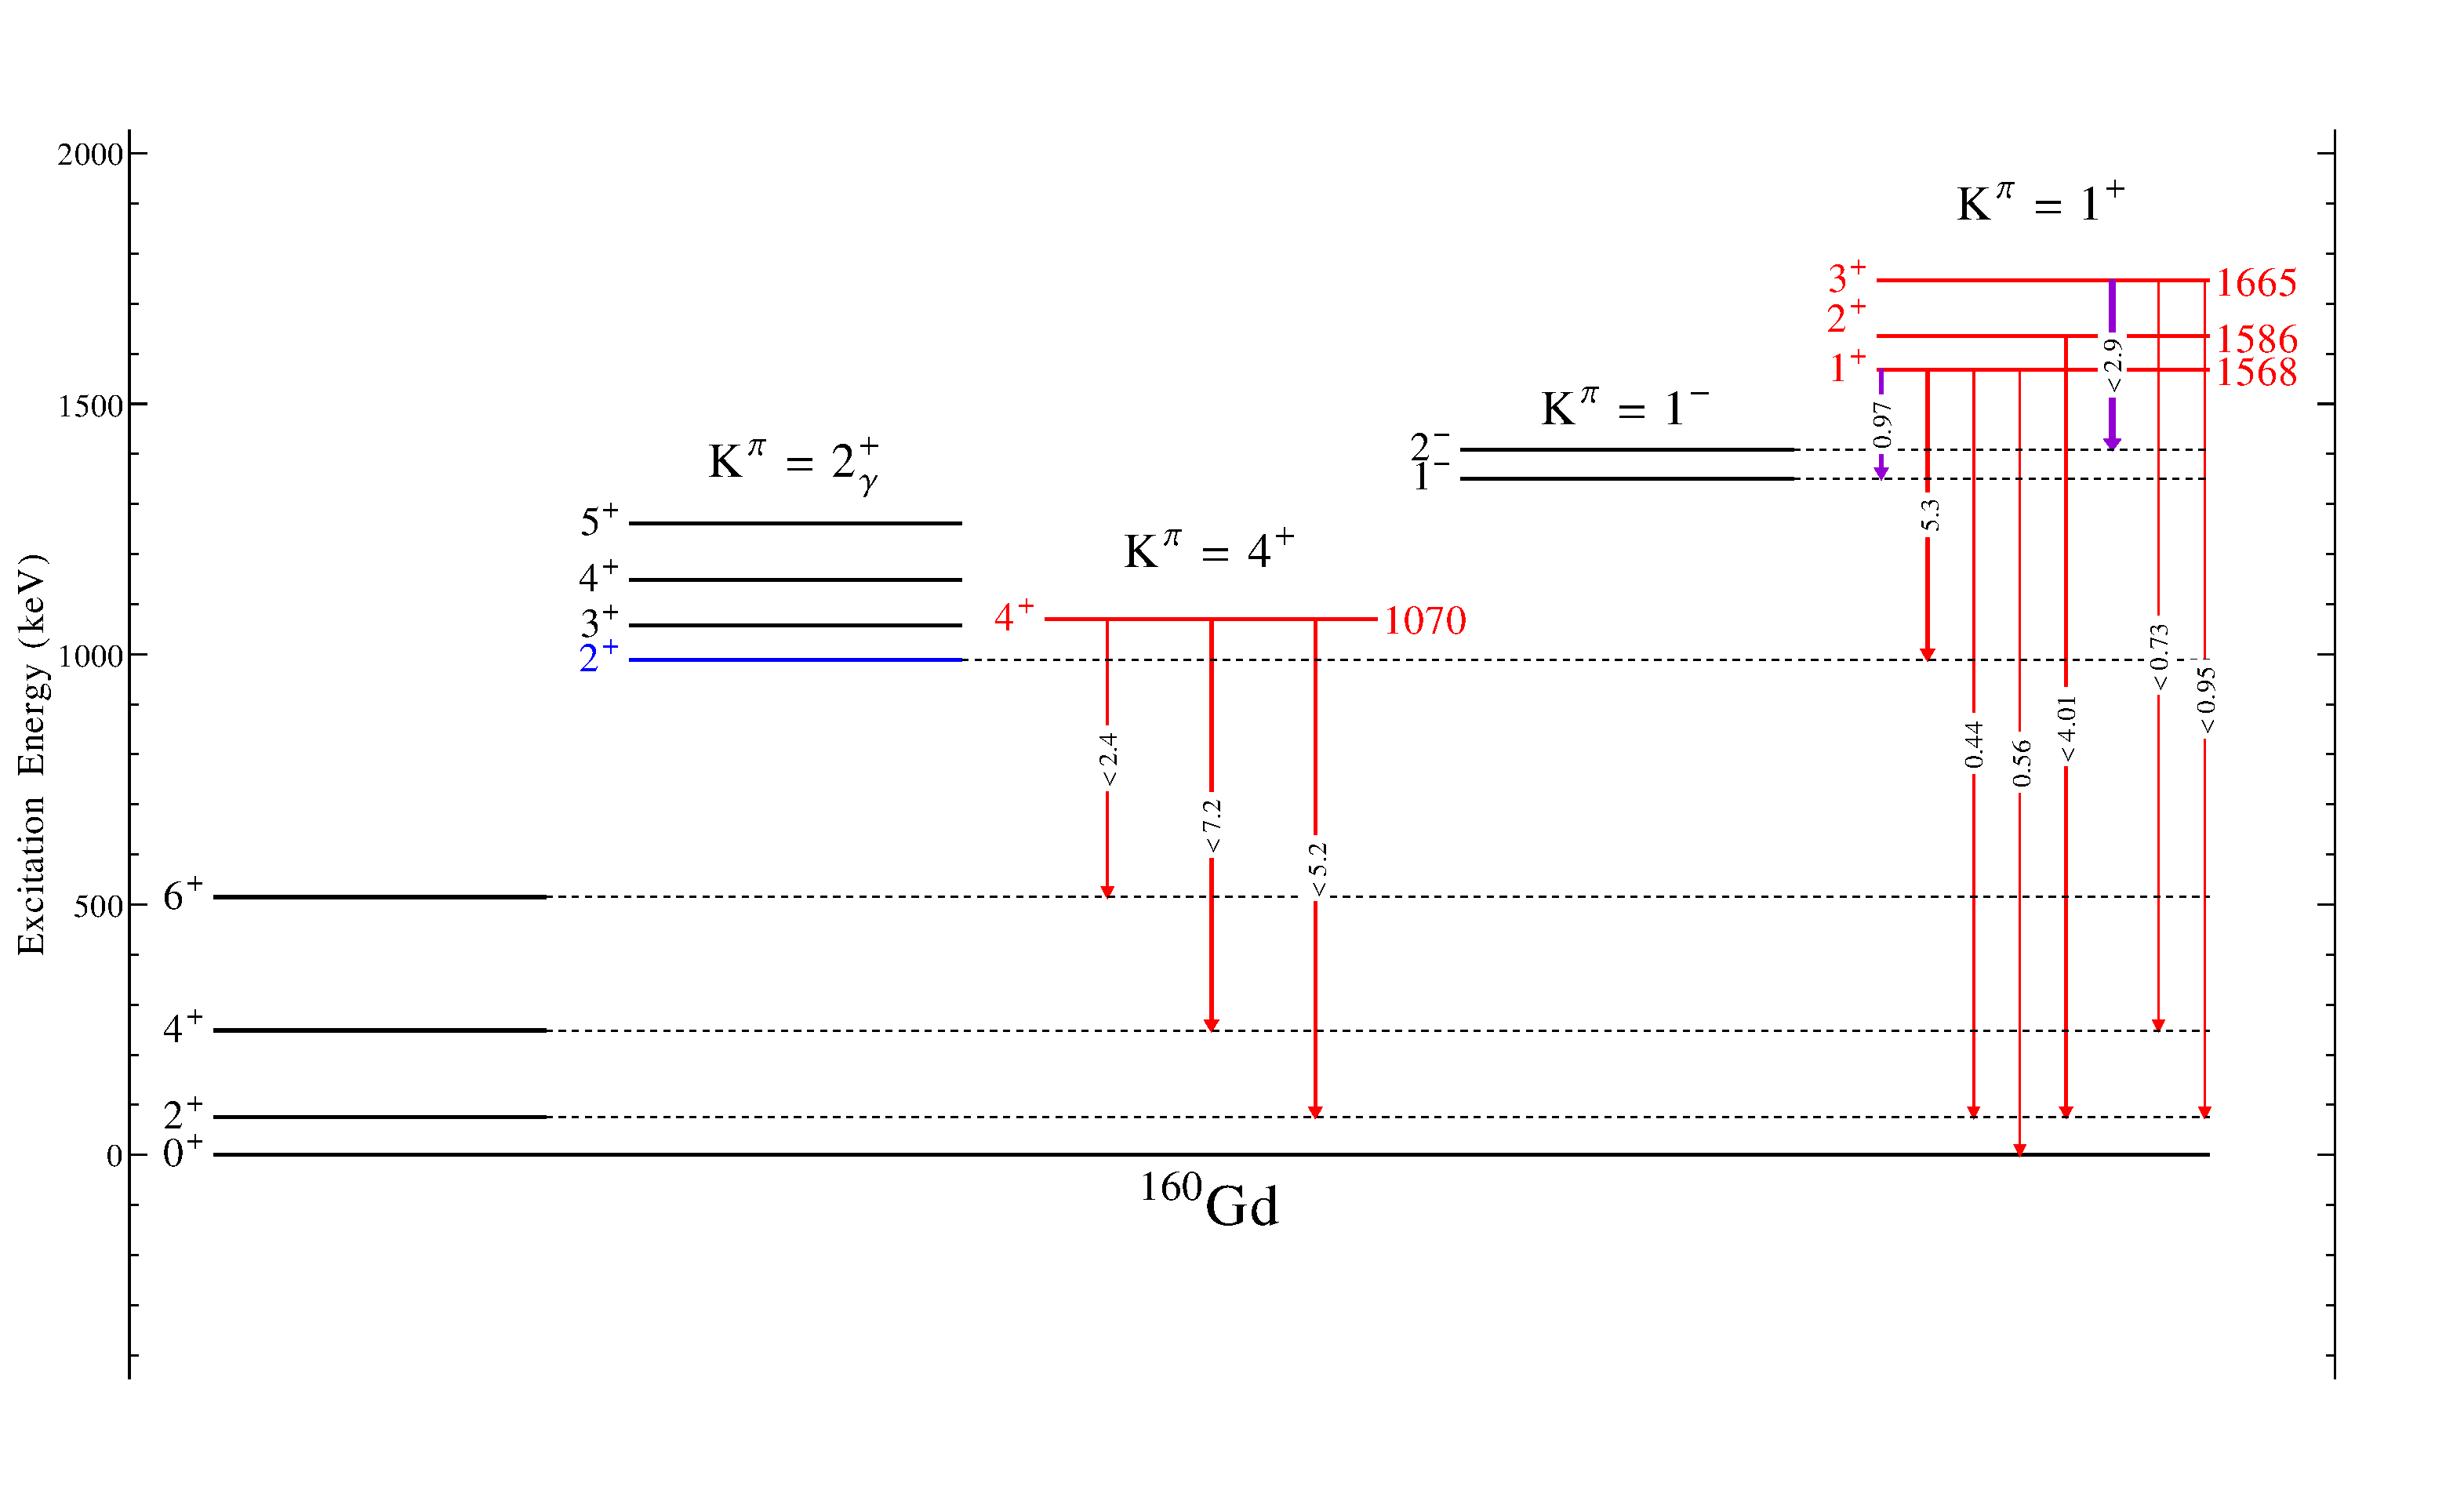
\includegraphics[width=0.99\textwidth]{figures/160Gd_posparity.pdf}
\caption{Level scheme showing the decays with calculated reduced transition probabilities for the K$^\pi$=4$^+$ and 1$^+$ bands in $^{160}$Gd. \label{fig:160Gd_posparity}}
\end{figure}
\end{center}


\subsubsection{K$^\pi$=4$^+$ Band as a Hexadecapole Vibration?}
The study of even, positive parity states continues into the interpretation of K$^\pi$=4$^+$ bands in deformed nuclei. We know from earlier assertions, that a $\gamma\gamma$ two-phonon vibration can have this K=4 angular momentum projection, but must also exhibit strongly collective decays to the $\gamma$-band, as each phonon must be `broken' individually, and in single steps. Any existence of this $\gamma\gamma$-type behavior in $^{160}$Gd is already dubious from energy considerations, as the expected energy for a harmonic two-phonon state should be roughly double the energy of the single-phonon counterpart. The E$_{\rm x}$=1070~keV state lies 100~keV above the $\gamma$-vibrational band, and in our measurement of the lifetime of this single 4$^+$ bandhead of the K$^\pi$=4$^+$ band, we find somewhat enhanced B(E2) transition probabilities to the ground state, with no de-excitations or preference of decay to the $\gamma$-vibrational band. This implies a lack of two-phonon characteristic in this excitation, and instead points towards a single phonon vibration of order $\lambda$=4; this hexadecapole nature is yet another expansion of the dynamic deformation in the geometric model set out by Bohr and Mottelson, and has been investigated in several works \cite{Burke_hexadecapole1994,Soloviev_QuadHex,Garrett_OctHex} for spherical and nearly-spherical nuclei. Again, much like the need for strong B(E3) radiation in determining octupole characteristics, the direct observation of E4 radiation depopulating K=4 bands would fully elucidate any hexadecapole nature in these states. We can, however, not say anything about hexadecapole vibrational characteristics in $^{160}$Gd with B(E2) measurements alone. Any assertions made would be tentative, as we are only able to extract a lower limit to the lifetime of this state at 1070~keV; further spectroscopy is needed to concretely say anything about the makeup of this state. That being said, Solviev has produced quasiparticle-phonon calculations that surmise this 4$^+$ state to be mostly hexadecapole in nature \cite{Soloviev_QuadHex}. Tangible experimental evidence for hexadecapole phonon behavior is nearly unprecedented in well-deformed nuclei, which our data could be one of the first signatures of this structure. This curious behavior in $^{160}$Gd begs further research, and, if this band is confirmed as a hexadecapole vibration built on top of the deformed ground state, it would be one of the lowest excitation energies of its kind, especially in a well-deformed nucleus.

\subsubsection{K$^\pi$=1$^+$ Band}
Our measurement of lifetimes for the K$^\pi$=1$^+$ band yields some interesting discussion in a potential quasiparticle-phonon coupling to either the established 1$^-$ band mentioned in \S \ref{sec:160Gd_negparity}, as well as the $\gamma$-vibrational band. We measured lifetimes for the 1$^+$, 2$^+$, and 3$^+$ members of this band, with several intraband transitions. Overall, we observe generally weak collectivity from members of this band to the ground state, with enhanced E1 transitions to the weakly collective K$^\pi$=1$^-$ band; normally and at first glance, this would imply some double-phonon collectivity, but this picture is obscured with a discretely preferential decay to the $\gamma$-vibrational band. This $\sim$5~W.u. B(E2) is hard to ignore, given its large branching ratio (30\%), especially in the context of strong intra-band transitions to known vibrational states in deformed nuclei. The most realistic outcome of interpretation of this band is of purely quasiparticle nature, where there is a strong implication that a majority of the corresponding nuclear wavefunction overlaps with the predominant configuration of the $\gamma$-vibrational band. Following in line with the major contributions to $\gamma$-vibrational bands in deformed nuclei from \cite{Casten_text}, we should expect and there is implication that significant overlap with the Nillson neutron wavefunctions of $\nu$($\frac{3}{2}$[521]+$\frac{1}{2}$[521]) exist for these states.


\begin{center}
\begin{figure}[h!]
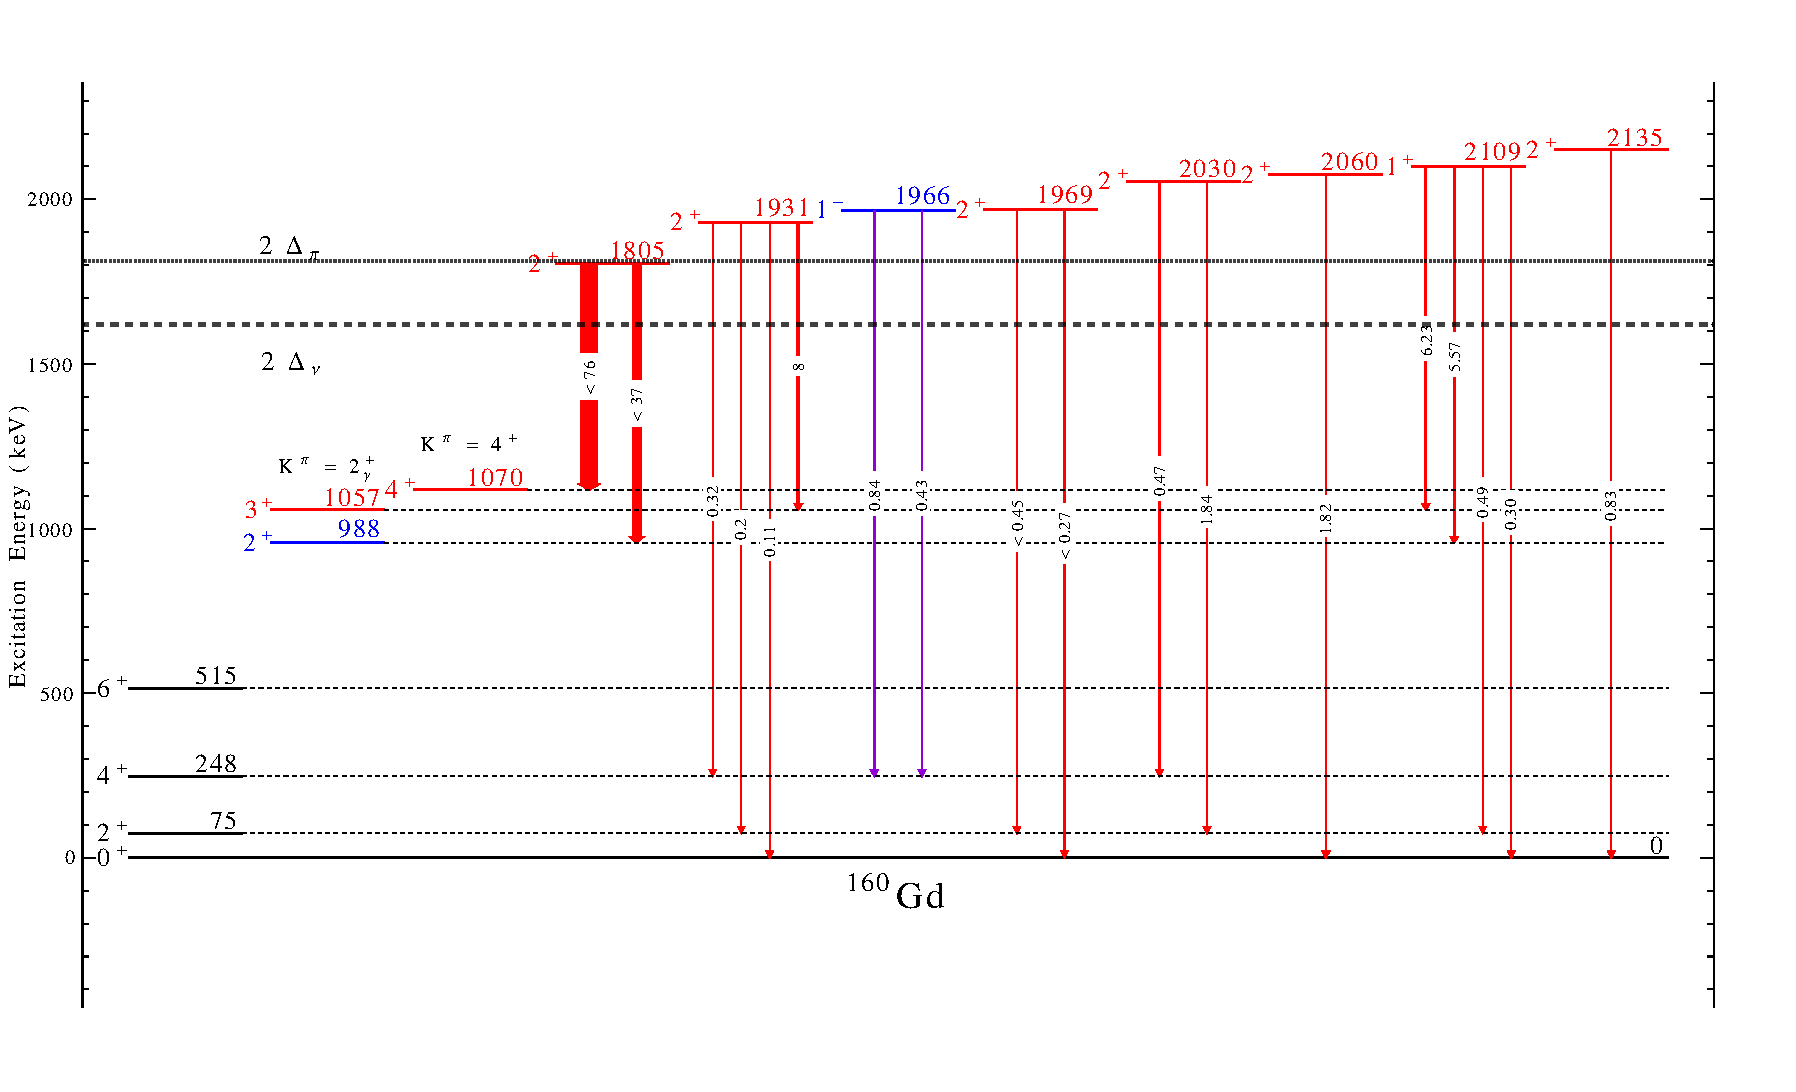
\includegraphics[width=0.99\textwidth]{figures/160Gd_Kunknown.pdf}
\caption{Level scheme showing the decays with calculated reduced transition probabilities for the levels that are not assigned to rotational bands in $^{160}$Gd. Note the neutron and proton pairing gaps drawn as dotted lines (2$\Delta_\nu\sim$1625~keV and 2$\Delta_\pi\sim$1810~keV). \label{fig:160Gd_Kunknown}}
\end{figure}
\end{center}

The inflated level density, uncertain spin-assignment, and higher probability for state-mixing to occur \cite{Casten_text} make band-assignments for these states well above the pairing gap increasingly difficult. That does not imply that the lifetimes measured are of diminished value; several instances of subtle nuclear structure exist at the higher energies studied in our experiments, such as the upcoming isovector dipole resonance in $^{162}$Dy. We have also not exhausted every possible two-phonon candidates in deformed nuclei, as the excessively rare `$\beta\gamma$'-type that would have a K-projection of 2$^+$. The signatures for this excitation follow the case for any two-phonon vibration, enhanced E2 transitions to a well-established vibrational band (in this case either a `$\gamma$' or `$\beta$' vibration). The best such candidate for a $\beta\gamma$ vibration is the 2$^+$ state at 1931~keV. We measure four decays from this state, and have a very well-defined lifetime from the Doppler Shifted $\gamma$ rays. The B(E2) probabilities here are very indicative of collective behavior built on top of the $\gamma$-band, with a collective 8~Weisskopf unit transition to the $\gamma$-band via a mostly ($\sim$92\%) E2 decay to the 3$^+$ member. To say that this is indeed a two-phonon collective vibration would be cavalier, of course, since we do not have complete and unambiguous assignment of the $\beta$ vibration. Since there are no other decays to the $\gamma$-vibrational band, we cannot make an Alaga comparison of transition strengths, and unfortunately, the large error (upper bound) shows the limiting power of DSAM near picosecond lifetimes. That all being said, given any rotational band assignment of this state, it could be a key asset in the search for a $\beta\gamma$-type vibration, and as we will see, the viability for anharmonic multiphonon configurations below an energy ratio of 2.

In the remaining states, we see some more of the mirrored assertions on any K$^\pi$=1$^+$ bands, with a strong coupling to the $\gamma$-vibrational band coming from another 1$^+$ state at 2109~keV. Of course, the macroscopic treatment of quadrupole vibrations by Bohr and Mottelson do not attribute any K$^\pi$=1$^+$ bands \cite{BohrMott_text}, so these states \textit{must} be of single- or multi-quasiparticle configurations. Yet again, the significantly preferred branching ratio and B(E2) strengths to the 2$^+$ band implies a dominant quasiparticle configuration involving the $\nu$($\frac{3}{2}$[521]+$\frac{1}{2}$[521]) shell using Nillson model considerations.

\subsection{Implications and Further Discussion}

In terms of a vibrational phonon model, we have measured new lifetimes for key states in $^{160}$Gd, the first being a potential (read: tentative) $\beta$-vibration existing as the lowest 0$^+$ state at 1379~keV. However, our assignment here is not conclusive enough to say for certain, as we only have upper limits to the collectivity, yet the potential for large B(E2) probabilities exists ($>$7~W.u. in strength for some transitions). This level of collectivity above 5~W.u. strength is in line with the assertions made by Garrett \cite{Garrett_betavib2001} on a concrete $\beta$-vibration assignment, however, this is only one possible interpretation, and again, we only have limits for measured B(E2)s in this lowest 0$^+$ band. This certainly does not spell doom for the feasability of the $\beta$ vibration, as we can still imagine a distinctly collective transition strength from the members of the 0$^+_2$ band. For multiphonon quadrupole vibrations in $^{160}$Gd, we do see a fairly definitive excitation of the $\gamma\gamma$-vibration as the third 0$^+$ state at 1558~keV via a highly collective transition from the 2$^+$ member of the band to the $\gamma$-vibrational band. Speaking of the $\gamma$-vibration, we measured lifetimes for the four lowest-lying members of the K$^\pi$=2$^+$ band that leads to the trademark $\sim$6-7~W.u. collectivity for the $\gamma$-vibrational band. 

The measurement of lifetimes in the negative parity bands yields some expected results from the systematic study of states in the region, with two well-defined octupole members (0$^-$ and 1$^-$), and a curious emerging decay pattern of K$^\pi$=2$^-$ bands to the $\gamma$-vibrational state. In all of these states, we measured distinctly inflated B(E1) transition probabilities, indicating some amount of dipole strength or asymmetry in the nuclear shape. In the case of the 0$^-$ and 1$^-$ bands, literature B(E3) values aid in the assessment of an octupole vibration built on top of the deformed ground state, and we have opened the question to find the remaining members of the vibration expected from the base Bohr-Mottelson formulation of the geometric model. 

Comparisons of the deduced B(E2) and B(E1) transition probabilities to the Alaga rules round out our discussion of the lifetimes measured in $^{160}$Gd. The ratios of our experimental transition probabilities and the Clebsch-Gordan coefficients squared are shown in Table \ref{tab:160Gd_ALAGA}, where we observe somewhat mixed agreement for the various bands in $^{160}$Gd. The comparison of our deduced B(E2) limits for the 0$^+_2$ band seems to be in stark disagreement, however, our measurement of upper limits of B(E2)s does not exclude agreement for \textit{any} combination of B(E2) value. For the 0$^+_3$ band, we note reasonable agreement (within the full range of uncertainty) for the Alaga comparisons; this includes both the decay channels to the K$^\pi$=0$^-$ octupole band and to the ground state band. The 2$^+_\gamma$ band is in reasonable agreement within error where we have convergent lifetimes (the 4$^+$ and 5$^+$ members), but we mirror the same assertions as the 0$^+_2$ band, where the disagreement for the upper limits of B(E2) do not offer much insight. Lastly, all of the negative parity band comparisons to the Alaga rules offer good agreement! Furthermore, the agreement of the K$^\pi$=2$^-$ band's measured B(E1)s imply that the K$^\pi$=2$^-$ assignment is valid, since a K$^\pi$=3$^-$ assignment would produce wildly variant Alaga expectations (\textit{e.g.} the ratio of Clebsch-Gordan coefficients in the K=3 case are 0.14, 0.05, 0.35 and 0.11 going down the table in the same order).

%good agreement 0_3, 2+ kinda, 0-, 1-, and 2-
%somewhat poor agreement with 0_2 and kinda 2+

\begin{table}[h!]
\begin{center}
\caption{ALAGA: $^{160}$GD \label{tab:160Gd_ALAGA}}

\begin{tabular}{llll}
K$^\pi$ & $\frac{J_i\rightarrow J_f^\prime}{J_i\rightarrow J_f^{\prime\prime}}$ & CG$^2$ & Exp \\ \hline \hline
K$^\pi$=0$^+_2$ & $\frac{2^+\rightarrow4^+}{2^+\rightarrow2^+}$ & 1.8 & 5.4 \\
                & $\frac{2^+\rightarrow4^+}{2^+\rightarrow0^+}$ & 2.6 & 19  \\
                & $\frac{2^+\rightarrow2^+}{2^+\rightarrow0^+}$ & 1.4 & 3.6 \\
                & $\frac{4^+\rightarrow6^+}{4^+\rightarrow4^+}$ & 1.8 & 4.1 \\ \hline
K$^\pi$=0$^+_3$ & $\frac{2^+\rightarrow3^-}{2^+\rightarrow1^-}$ & 1.5 & 1.1 \\
                & $\frac{2^+\rightarrow2^+}{2^+\rightarrow0^+}$ & 1.4 & 0.8 \\ \hline
K$^\pi$=2$^+_\gamma$ & $\frac{2^+\rightarrow2^+}{2^+\rightarrow0^+}$ & 1.4 & 0.3 \\ 
                     & $\frac{3^+\rightarrow4^+}{3^+\rightarrow2^+}$ & 0.4 & 0.01 \\
                     & $\frac{4^+\rightarrow4^+}{4^+\rightarrow2^+}$ & 2.9 & 4.2 \\
                     & $\frac{5^+\rightarrow6^+}{5^+\rightarrow4^+}$ & 0.6 & 0.9 \\ \hline
K$^\pi$=0$^-$ & $\frac{1^-\rightarrow2^+}{1^-\rightarrow0^+}$ & 2.0 & 1.8 \\
              & $\frac{3^-\rightarrow4^+}{3^-\rightarrow2^+}$ & 1.3 & 0.9 \\ \hline
K$^\pi$=1$^-$ & $\frac{1^-\rightarrow2^+}{1^-\rightarrow0^+}$ & 0.5 & 0.7 \\ \hline
K$^\pi$=2$^-$ & $\frac{3^-\rightarrow4^+_\gamma}{3^-\rightarrow3^+_\gamma}$ & 1.3 & 1.0 \\
              & $\frac{3^-\rightarrow4^+_\gamma}{3^-\rightarrow2^+_\gamma}$ & 1.8 & 1.4  \\
              & $\frac{3^-\rightarrow3^+_\gamma}{3^-\rightarrow2^+_\gamma}$ & 1.4 & 1.3 \\
              & $\frac{4^-\rightarrow5^+_\gamma}{4^-\rightarrow3^+_\gamma}$ & 1.4 & 1.4 \\
\end{tabular}\\
\end{center}
Alaga comparisons of B($\pi\ell$) transition probabilities in $^{160}$Gd measured in our experiments.
\end{table}

